\documentclass{article}
\usepackage{tikz}

\begin{document}

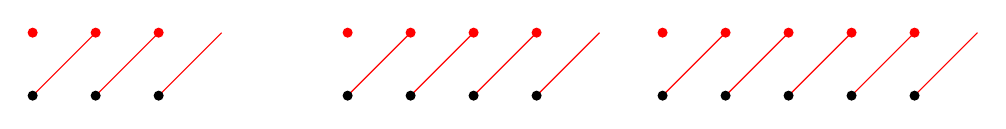
\begin{tikzpicture}[scale=0.8]
    % Step 1
    \draw[red] (0,0) -- (1,1);
    \draw[red] (1,0) -- (2,1);
    \draw[red] (2,0) -- (3,1);
    \filldraw[black] (0,0) circle (2pt);
    \filldraw[black] (1,0) circle (2pt);
    \filldraw[black] (2,0) circle (2pt);
    \filldraw[red] (0,1) circle (2pt);
    \filldraw[red] (1,1) circle (2pt);
    \filldraw[red] (2,1) circle (2pt);

    % Step 2
    \begin{scope}[xshift=5cm]
        \draw[red] (0,0) -- (1,1);
        \draw[red] (1,0) -- (2,1);
        \draw[red] (2,0) -- (3,1);
        \draw[red] (3,0) -- (4,1);
        \filldraw[black] (0,0) circle (2pt);
        \filldraw[black] (1,0) circle (2pt);
        \filldraw[black] (2,0) circle (2pt);
        \filldraw[black] (3,0) circle (2pt);
        \filldraw[red] (0,1) circle (2pt);
        \filldraw[red] (1,1) circle (2pt);
        \filldraw[red] (2,1) circle (2pt);
        \filldraw[red] (3,1) circle (2pt);
    \end{scope}

    % Step 3
    \begin{scope}[xshift=10cm]
        \draw[red] (0,0) -- (1,1);
        \draw[red] (1,0) -- (2,1);
        \draw[red] (2,0) -- (3,1);
        \draw[red] (3,0) -- (4,1);
        \draw[red] (4,0) -- (5,1);
        \filldraw[black] (0,0) circle (2pt);
        \filldraw[black] (1,0) circle (2pt);
        \filldraw[black] (2,0) circle (2pt);
        \filldraw[black] (3,0) circle (2pt);
        \filldraw[black] (4,0) circle (2pt);
        \filldraw[red] (0,1) circle (2pt);
        \filldraw[red] (1,1) circle (2pt);
        \filldraw[red] (2,1) circle (2pt);
        \filldraw[red] (3,1) circle (2pt);
        \filldraw[red] (4,1) circle (2pt);
    \end{scope}
\end{tikzpicture}

\end{document}